% TODO translate
\subsection{Chiffrement simple utilisant un masque XOR}
\label{XOR_mask_1}

J'ai trouvé un vieux jeu de fiction interactif en plongeant profondément dans \emph{if-archive}\footnote{\url{http://www.ifarchive.org/}}:

\begin{lstlisting}
The New Castle v3.5 - Text/Adventure Game
in the style of the original Infocom (tm)
type games, Zork, Collosal Cave (Adventure),
etc.  Can you solve the mystery of the
abandoned castle?
Shareware from Software Customization.
Software Customization [ASP] Version 3.5 Feb. 2000
\end{lstlisting}

Il est téléchargeable
\href{\RepoURL/ff/XOR/mask_1/files/newcastle.tgz}{ici}.

Il y a un fichier à l'intérieur (appelé \emph{castle.dbf}) qui est visiblement chiffré,
mais pas avec un vrai algorithme de crypto, qui n'est pas non plus compressé, il
s'agit plutôt de quelque chose de plus simple.
Je ne vais même pas mesurer le niveau d'entropie (\myref{entropy}) du fichier, car
je suis sûr qu'il est bas.
Voici à quoi il ressemble dans Midnight Commander:

\begin{figure}[H]
\centering
\myincludegraphics{ff/XOR/mask_1/mc_encrypted.png}
\caption{Fichier chiffré dans Midnight Commander}
\end{figure}

Le fichier chiffré peut être téléchargé ici:
\href{\RepoURL/ff/XOR/mask_1/files/castle.dbf.bz2}.

Sera-t-il possible de le décrypter sans accéder au programme, en utilisant juste ce
fichier?

Il y a clairement un pattern visible de chaînes répétées.
Si un simple chiffrement avec un masque XOR a été appliqué, une répétition de telles
chaînes en est une signature notable, car, il y avait probablement de longues
suites (lacunes\footnote{Comme dans \url{https://en.wikipedia.org/wiki/Lacuna_(manuscripts)}})
d'octets à zéro, qui, à tour de rôle, sont présentes dans de nombreux
fichiers exécutables, tout comme dans des fichiers de données binaires.

\myindex{UNIX!xxd}
Ici, je vais afficher le début du fichier en utilisant l'utilitaire UNIX \emph{xxd}:

\lstinputlisting{ff/XOR/mask_1/xxd_result.txt}

Concentrons-nous sur la chaîne visible \TT{iubgv} se répétant.
En regardant ce dump, nous voyons clairement que la période de l'occurrence de la chaîne
est 0x51 ou 81.
La taille du fichier est 1658961, et est divisible par 81 (et il y a donc 20481 blocs).

Maintenant, je vais utiliser Mathematica pour l'analyse, y a-t-il des blocs de 81
octets se répètant dans le fichier?
Je vais séparer le fichier d'entrée en blocs de 81 octets et ensuite utiliser la fonction
\emph{Tally[]}\footnote{\url{https://reference.wolfram.com/language/ref/Tally.html}}
qui compte simplement combien de fois un élément était présent dans la liste en entrée.
La sortie de Tally n'est pas triée, donc je vais ajouter la fonction \emph{Sort[]}
pour trier le nombre d'occurrences par ordre décroissant.

\begin{lstlisting}[style=custommath]
input = BinaryReadList["/home/dennis/.../castle.dbf"];

blocks = Partition[input, 81];

stat = Sort[Tally[blocks], #1[[2]] > #2[[2]] &]
\end{lstlisting}

Et voici la sortie:

\begin{lstlisting}[style=custommath]
{{{80, 103, 2, 116, 113, 102, 118, 25, 99, 8, 19, 23, 116, 125, 107, 
   25, 99, 109, 114, 102, 14, 121, 115, 31, 9, 117, 113, 111, 5, 4, 
   127, 28, 122, 101, 8, 110, 14, 18, 124, 106, 16, 20, 104, 119, 8, 
   109, 26, 106, 9, 97, 13, 99, 15, 119, 20, 105, 117, 98, 103, 118, 
   1, 126, 29, 97, 122, 17, 15, 114, 110, 3, 5, 125, 125, 99, 126, 
   119, 102, 30, 122, 2, 117}, 1739}, 
{{80, 100, 2, 116, 113, 102, 118, 25, 99, 8, 19, 23, 116, 
   125, 107, 25, 99, 109, 114, 102, 14, 121, 115, 31, 9, 117, 113, 
   111, 5, 4, 127, 28, 122, 101, 8, 110, 14, 18, 124, 106, 16, 20, 
   104, 119, 8, 109, 26, 106, 9, 97, 13, 99, 15, 119, 20, 105, 117, 
   98, 103, 118, 1, 126, 29, 97, 122, 17, 15, 114, 110, 3, 5, 125, 
   125, 99, 126, 119, 102, 30, 122, 2, 117}, 1422}, 
{{80, 101, 2, 116, 113, 102, 118, 25, 99, 8, 19, 23, 116, 
   125, 107, 25, 99, 109, 114, 102, 14, 121, 115, 31, 9, 117, 113, 
   111, 5, 4, 127, 28, 122, 101, 8, 110, 14, 18, 124, 106, 16, 20, 
   104, 119, 8, 109, 26, 106, 9, 97, 13, 99, 15, 119, 20, 105, 117, 
   98, 103, 118, 1, 126, 29, 97, 122, 17, 15, 114, 110, 3, 5, 125, 
   125, 99, 126, 119, 102, 30, 122, 2, 117}, 1012},
{{80, 120, 2, 116, 113, 102, 118, 25, 99, 8, 19, 23, 116, 
   125, 107, 25, 99, 109, 114, 102, 14, 121, 115, 31, 9, 117, 113, 
   111, 5, 4, 127, 28, 122, 101, 8, 110, 14, 18, 124, 106, 16, 20, 
   104, 119, 8, 109, 26, 106, 9, 97, 13, 99, 15, 119, 20, 105, 117, 
   98, 103, 118, 1, 126, 29, 97, 122, 17, 15, 114, 110, 3, 5, 125, 
   125, 99, 126, 119, 102, 30, 122, 2, 117}, 377},

...

{{80, 2, 74, 49, 113, 21, 62, 88, 39, 71, 68, 23, 63, 51, 36, 78, 48, 
   108, 114, 102, 14, 121, 115, 31, 9, 117, 113, 111, 5, 4, 127, 28, 
   122, 101, 8, 110, 14, 18, 124, 106, 16, 20, 104, 119, 8, 109, 26, 
   106, 9, 97, 13, 99, 15, 119, 20, 105, 117, 98, 103, 118, 1, 126, 
   29, 97, 122, 17, 15, 114, 110, 3, 5, 125, 125, 99, 126, 119, 102, 
   30, 122, 2, 117}, 1},
{{80, 1, 74, 59, 113, 45, 56, 86, 52, 91, 19, 64, 60, 60, 63, 
   25, 38, 59, 59, 42, 14, 53, 38, 77, 66, 38, 113, 38, 75, 4, 43, 84,
    63, 101, 64, 43, 79, 64, 40, 57, 16, 91, 46, 119, 69, 40, 84, 117,
    9, 97, 13, 99, 15, 119, 20, 105, 117, 98, 103, 118, 1, 126, 29, 
   97, 122, 17, 15, 114, 110, 3, 5, 125, 125, 99, 126, 119, 102, 30, 
   122, 2, 117}, 1},
{{80, 2, 74, 49, 113, 49, 51, 92, 39, 8, 92, 81, 116, 62, 57, 
   80, 46, 40, 114, 36, 75, 56, 33, 76, 9, 55, 56, 59, 81, 65, 45, 28,
    60, 55, 93, 39, 90, 28, 124, 106, 16, 20, 104, 119, 8, 109, 26, 
   106, 9, 97, 13, 99, 15, 119, 20, 105, 117, 98, 103, 118, 1, 126, 
   29, 97, 122, 17, 15, 114, 110, 3, 5, 125, 125, 99, 126, 119, 102, 
   30, 122, 2, 117}, 1}}
\end{lstlisting}

La sortie de Tally est une liste de paires, chaque paire a un bloc de 81 octets et
le nombre de fois qu'il apparaît dans le fichier.
Nous voyons que le bloc le plus fréquent est le premier, il est apparu 1739 fois.
Le second apparaît 1422 fois. Puis les autres: 1012 fois, 377 fois, etc.
Les blocs de 81 octets qui ne sont apparus qu'une fois sont à la fin de la sortie.

Essayons de comparer ces blocs. Le premier et le second.
Y a-t-il une fonction dans Mathematica qui compare les listes/tableaux?
Certainement qu'il y en a une, mais dans un but didactique, je vais utiliser
l'opération XOR pour la comparaison.
En effet: si les octets dans deux tableaux d'entrée sont identiques, le résultat
du XOR est 0. Si ils sont différents, le résultat sera différent de zéro.

Comparons le premier bloc (qui apparaît 1739 fois) et le second (qui apparaît 1422 fois):

\begin{lstlisting}[style=custommath]
In[]:= BitXor[stat[[1]][[1]], stat[[2]][[1]]]
Out[]= {0, 3, 0, 0, 0, 0, 0, 0, 0, 0, 0, 0, 0, 0, 0, 0, 0, 0, 0, \
0, 0, 0, 0, 0, 0, 0, 0, 0, 0, 0, 0, 0, 0, 0, 0, 0, 0, 0, 0, 0, 0, 0, \
0, 0, 0, 0, 0, 0, 0, 0, 0, 0, 0, 0, 0, 0, 0, 0, 0, 0, 0, 0, 0, 0, 0, \
0, 0, 0, 0, 0, 0, 0, 0, 0, 0, 0, 0, 0, 0, 0, 0}
\end{lstlisting}

Ils ne diffèrent que par le second octet.

Comparons le second bloc (qui apparaît 1422 fois) et le troisième (qui apparaît 1012 fois):

\begin{lstlisting}[style=custommath]
In[]:= BitXor[stat[[2]][[1]], stat[[3]][[1]]]
Out[]= {0, 1, 0, 0, 0, 0, 0, 0, 0, 0, 0, 0, 0, 0, 0, 0, 0, 0, 0, \
0, 0, 0, 0, 0, 0, 0, 0, 0, 0, 0, 0, 0, 0, 0, 0, 0, 0, 0, 0, 0, 0, 0, \
0, 0, 0, 0, 0, 0, 0, 0, 0, 0, 0, 0, 0, 0, 0, 0, 0, 0, 0, 0, 0, 0, 0, \
0, 0, 0, 0, 0, 0, 0, 0, 0, 0, 0, 0, 0, 0, 0, 0}
\end{lstlisting}

Ils ne diffèrent également que par le second octet.

Quoiqu'il en soit, essayons d'utiliser le bloc qui apparaît le plus comme une clef
XOR et essayons de déchiffrer les quatre premiers blocs de 81 octets dans le fichier:

\begin{lstlisting}[style=custommath]
In[]:= key = stat[[1]][[1]]
Out[]= {80, 103, 2, 116, 113, 102, 118, 25, 99, 8, 19, 23, 116, \
125, 107, 25, 99, 109, 114, 102, 14, 121, 115, 31, 9, 117, 113, 111, \
5, 4, 127, 28, 122, 101, 8, 110, 14, 18, 124, 106, 16, 20, 104, 119, \
8, 109, 26, 106, 9, 97, 13, 99, 15, 119, 20, 105, 117, 98, 103, 118, \
1, 126, 29, 97, 122, 17, 15, 114, 110, 3, 5, 125, 125, 99, 126, 119, \
102, 30, 122, 2, 117}

In[]:= ToASCII[val_] := If[val == 0, " ", FromCharacterCode[val, "PrintableASCII"]]

In[]:= DecryptBlockASCII[blk_] := Map[ToASCII[#] &, BitXor[key, blk]]

In[]:= DecryptBlockASCII[blocks[[1]]]
Out[]= {" ", " ", " ", " ", " ", " ", " ", " ", " ", " ", " ", " \
", " ", " ", " ", " ", " ", " ", " ", " ", " ", " ", " ", " ", " ", " \
", " ", " ", " ", " ", " ", " ", " ", " ", " ", " ", " ", " ", " ", " \
", " ", " ", " ", " ", " ", " ", " ", " ", " ", " ", " ", " ", " ", " \
", " ", " ", " ", " ", " ", " ", " ", " ", " ", " ", " ", " ", " ", " \
", " ", " ", " ", " ", " ", " ", " ", " ", " ", " ", " ", " ", " "}

In[]:= DecryptBlockASCII[blocks[[2]]]
Out[]= {" ", "e", "H", "E", " ", "W", "E", "E", "D", " ", "O", \
"F", " ", "C", "R", "I", "M", "E", " ", "B", "E", "A", "R", "S", " ", \
"B", "I", "T", "T", "E", "R", " ", "F", "R", "U", "I", "T", "?", \
" ", " ", " ", " ", " ", " ", " ", " ", " ", " ", " ", " ", " ", " ", \
" ", " ", " ", " ", " ", " ", " ", " ", " ", " ", " ", " ", " ", " ", \
" ", " ", " ", " ", " ", " ", " ", " ", " ", " ", " ", " ", " ", " ", \
" "}

In[]:= DecryptBlockASCII[blocks[[3]]]
Out[]= {" ", "?", " ", " ", " ", " ", " ", " ", " ", " ", " \
", " ", " ", " ", " ", " ", " ", " ", " ", " ", " ", " ", " ", " ", " \
", " ", " ", " ", " ", " ", " ", " ", " ", " ", " ", " ", " ", " ", " \
", " ", " ", " ", " ", " ", " ", " ", " ", " ", " ", " ", " ", " ", " \
", " ", " ", " ", " ", " ", " ", " ", " ", " ", " ", " ", " ", " ", " \
", " ", " ", " ", " ", " ", " ", " ", " ", " ", " ", " ", " ", " ", " \
"}

In[]:= DecryptBlockASCII[blocks[[4]]]
Out[]= {" ", "f", "H", "O", " ", "K", "N", "O", "W", "S", " ", \
"W", "H", "A", "T", " ", "E", "V", "I", "L", " ", "L", "U", "R", "K", \
"S", " ", "I", "N", " ", "T", "H", "E", " ", "H", "E", "A", "R", "T", \
"S", " ", "O", "F", " ", "M", "E", "N", "?", " ", " ", " ", " ", \
" ", " ", " ", " ", " ", " ", " ", " ", " ", " ", " ", " ", " ", " ", \
" ", " ", " ", " ", " ", " ", " ", " ", " ", " ", " ", " ", " ", " ", \
" "}
\end{lstlisting}

(J'ai remplacé les caractères non imprimables par \q{?}.)

Donc nous voyons que le premier et le troisième blocs sont vides (ou presque vide),
mais le second et le quatrième comportent clairement des mots/phrases en anglais.
Ils semble que notre hypothèse à propos de la clef soit correct (au moins en partie).
Cala signifie que le bloc de 81 octets qui apparaît le plus souvent dans le fichier
peut être trouvé à des endroits comportant des séries d'octets à zéro ou quelque
chose comme ça.

Essayons de déchiffrer le fichier entier:

\begin{lstlisting}[style=custommath]
DecryptBlock[blk_] := BitXor[key, blk]

decrypted = Map[DecryptBlock[#] &, blocks];

BinaryWrite["/home/dennis/.../tmp", Flatten[decrypted]]

Close["/home/dennis/.../tmp"]
\end{lstlisting}

\begin{figure}[H]
\centering
\myincludegraphics{ff/XOR/mask_1/mc_decrypted1.png}
\caption{Fichier déchiffré dans Midnight Commander, 1er essai}
\end{figure}

Ceci ressemble a des sortes de phrases en anglais d'un jeu, mais quelque chose ne
va pas.
Tout d'abord, la casse est inversée: les phrases et certains mots commence avec une
minuscule, tandis que d'autres caractères sont en majuscule.
De plus, certaines phrases commencent avec une mauvaise lettre.
Regardez la toute première phrase: \q{eHE WEED OF CRIME BEARS BITTER FRUIT}.
Que signifie \q{eHE}? Ne devrait-on pas avoir \q{tHE} ici?
Est-il possible que notre clef de déchiffrement ait un mauvais octet à cet endroit?

Regardons à nouveau le second bloc dans le fichier, la clef et le résultat décrypté:

\begin{lstlisting}[style=custommath]
In[]:= blocks[[2]]
Out[]= {80, 2, 74, 49, 113, 49, 51, 92, 39, 8, 92, 81, 116, 62, \
57, 80, 46, 40, 114, 36, 75, 56, 33, 76, 9, 55, 56, 59, 81, 65, 45, \
28, 60, 55, 93, 39, 90, 28, 124, 106, 16, 20, 104, 119, 8, 109, 26, \
106, 9, 97, 13, 99, 15, 119, 20, 105, 117, 98, 103, 118, 1, 126, 29, \
97, 122, 17, 15, 114, 110, 3, 5, 125, 125, 99, 126, 119, 102, 30, \
122, 2, 117}

In[]:= key
Out[]= {80, 103, 2, 116, 113, 102, 118, 25, 99, 8, 19, 23, 116, \
125, 107, 25, 99, 109, 114, 102, 14, 121, 115, 31, 9, 117, 113, 111, \
5, 4, 127, 28, 122, 101, 8, 110, 14, 18, 124, 106, 16, 20, 104, 119, \
8, 109, 26, 106, 9, 97, 13, 99, 15, 119, 20, 105, 117, 98, 103, 118, \
1, 126, 29, 97, 122, 17, 15, 114, 110, 3, 5, 125, 125, 99, 126, 119, \
102, 30, 122, 2, 117}

In[]:= BitXor[key, blocks[[2]]]
Out[]= {0, 101, 72, 69, 0, 87, 69, 69, 68, 0, 79, 70, 0, 67, 82, \
73, 77, 69, 0, 66, 69, 65, 82, 83, 0, 66, 73, 84, 84, 69, 82, 0, 70, \
82, 85, 73, 84, 14, 0, 0, 0, 0, 0, 0, 0, 0, 0, 0, 0, 0, 0, 0, 0, 0, \
0, 0, 0, 0, 0, 0, 0, 0, 0, 0, 0, 0, 0, 0, 0, 0, 0, 0, 0, 0, 0, 0, 0, \
0, 0, 0, 0}
\end{lstlisting}

L'octet chiffré est 2, l'octet de la clef est 103, $2 \oplus 103=101$ et 101 est
le code ASCII du caractère \q{e}.
A quoi devrait être égal l'octet de la clef, afin que le code ASCII résultant soit
116 (pour le caractère \q{t})?
$2 \oplus 116=118$, mettons 118 comme second octet de la clef \dots

\begin{lstlisting}[style=custommath]
key = {80, 118, 2, 116, 113, 102, 118, 25, 99, 8, 19, 23, 116, 125, 
  107, 25, 99, 109, 114, 102, 14, 121, 115, 31, 9, 117, 113, 111, 5, 
  4, 127, 28, 122, 101, 8, 110, 14, 18, 124, 106, 16, 20, 104, 119, 8,
   109, 26, 106, 9, 97, 13, 99, 15, 119, 20, 105, 117, 98, 103, 118, 
  1, 126, 29, 97, 122, 17, 15, 114, 110, 3, 5, 125, 125, 99, 126, 119,
   102, 30, 122, 2, 117}
\end{lstlisting}

\dots et déchiffrons le fichier à nouveau.

\begin{figure}[H]
\centering
\myincludegraphics{ff/XOR/mask_1/mc_decrypted2.png}
\caption{Fichier déchiffré dans Midnight Commander, 2nd essai}
\end{figure}

Ouah, maintenant, la grammaire est correcte, toutes les phrases commencent avec une lettre
correcte.
Mais encore, l'inversion de la casse est suspecte.
Pourquoi est-ce que le développeur les aurait écrites de cette façon?
Peut-être que notre clef est toujours incorrecte?

En regardant la table ASCII, nous pouvons remarquer que les codes des lettres majuscules
et des minuscules ne diffèrent que d'un bit (6ème bit en partant de 1, 0b100000):

\begin{figure}[H]
\centering
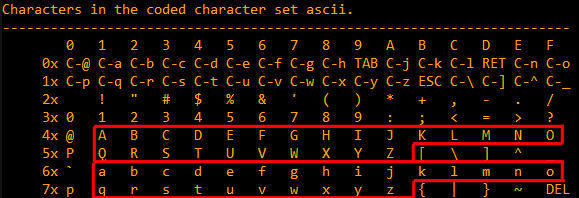
\includegraphics[width=0.8\textwidth]{ascii.png}
\caption{table \ac{ASCII} 7-bit dans Emacs}
\end{figure}

Cet octet avec seul le 6ème bit mis est 32 au format décimal.
Mais 32 est le code ASCII de l'espace!

En effet, on peut changer la casse juste en XOR-ant le code ASCII d'un caractère
avec 32 (plus à ce sujet: \myref{toupper_bit}).

Est-ce possible que les parties vides dans le fichier ne soient pas des octets à zéro,
mais plutôt des espaces?
Modifions notre clef XOR encore une fois (je vais appliquer Un XOR avec 32 à chaque
octet de la clef):

\begin{lstlisting}[style=custommath]
(* "32" is scalar and "key" is vector, but that's OK *)

In[]:= key3 = BitXor[32, key]
Out[]= {112, 86, 34, 84, 81, 70, 86, 57, 67, 40, 51, 55, 84, 93, 75, \
57, 67, 77, 82, 70, 46, 89, 83, 63, 41, 85, 81, 79, 37, 36, 95, 60, \
90, 69, 40, 78, 46, 50, 92, 74, 48, 52, 72, 87, 40, 77, 58, 74, 41, \
65, 45, 67, 47, 87, 52, 73, 85, 66, 71, 86, 33, 94, 61, 65, 90, 49, \
47, 82, 78, 35, 37, 93, 93, 67, 94, 87, 70, 62, 90, 34, 85}

In[]:= DecryptBlock[blk_] := BitXor[key3, blk]
\end{lstlisting}

Déchiffrons à nouveau le fichier d'entrée:

\begin{figure}[H]
\centering
\myincludegraphics{ff/XOR/mask_1/mc_decrypted.png}
\caption{Fichier déchiffré dans Midnight Commander, essai final}
\end{figure}

(Le fichier déchiffré est disponible
\href{\RepoURL/ff/XOR/mask_1/files/decrypted.dat.bz2}{ici}.)

Ceci est indiscutablement un fichier source correct.
Oh, et nous voyons des nombres au début de chaque bloc. Ça doit être la source de
notre clef XOR erronée.
Il semble que le bloc de 81 octets le plus fréquent dans le fichier soit un bloc
rempli avec des espaces et contenant le caractère \q{1} à la place du second octet.
En effet, d'une façon ou d'une autre, de nombreux blocs sont entrelacés avec celui-ci.

Peut-être est-ce une sorte de remplissage pour les phrases/messages courts?
D'autres blocs de 81 octets sont aussi remplis avec des blocs d'espaces, mais avec
un chiffre différent, ainsi, ils ne diffèrent que du second octet.

C'est tout! Maintenant nous pouvons écrire un utilitaire pour chiffrer à nouveau le
fichier, et peut-être le modifier avant.

Le fichier notebook de Mathematica est téléchargeable 
\href{\RepoURL/ff/XOR/mask_1/files/XOR_mask_1.nb}{ici}.

Résumé: un tel chiffrement avec XOR n'est pas robuste du tout. Le développeur du jeu
escomptait, probablement, empêcher les joueurs de chercher des informations sur le
jeu, mais rien de plus sérieux.
Néanmoins, un tel chiffrement est très populaire du fait de sa simplicité et de nombreux
rétro-ingénieurs sont traditionnellement familier avec.

